\chapter{Incompressible flow passing a step}
\label{tut:stepflow}

\section{Solution with linear triangles}

\modinfo{Directory}{FlowStepIncompressible}
\modinfo{Solvers}{\Idx{FlowSolve}}
\modinfo{Tools}{\Idx{ElmerFront}}
\modinfo{Dimensions}{2D, Steady-state}


\subsection*{Case definition}

A fluid, flowing past a step (see figure~\ref{fg:struct2}), has the density
1~kg/m$�$ and viscosity 0.01~kg/ms. The velocity of the fluid on the 
incoming boundary $\Gamma_6$ in the x-direction is 1~m/s and in 
the y-direction 0~m/s (see figure~\ref{fg:struct2}). On the outcoming boundary 
$\Gamma_4$ the velocity is 0~m/s in the y-direction and the pressure
is 0~Pa. The problem is to solve the velocity field and the pressure 
change in $\Omega$.

\begin{figure}[h]
\centering
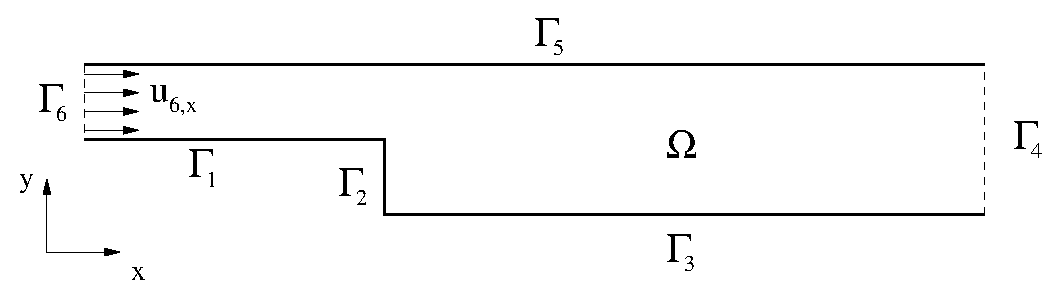
\includegraphics[width=100mm]{Body1}
\caption{Step.}\label{fg:struct2}
\end{figure}

Mathematically the problem to be solved is
\begin{equation}
\left \{
\begin{array}{rccl}
- \nabla \cdot (2 \mu \overline{\overline{\varepsilon}}) + \rho 
\vec{u} \cdot \nabla \vec{u} + \nabla p & = & 0 & \mbox{ in } \Omega \\
\nabla \cdot \vec{u} & = & 0 & \mbox{ in } \Omega \\
\end{array}
\right .
\end{equation}
with the boundary conditions
\begin{equation}
\left \{
\begin{array}{rccl}
\vec{u}_{x} & = & 1 & \mbox{ on } \Gamma_6 \\
\vec{u}_{x} & = & 0 & \mbox{ on } \Gamma_i ,\: i=1,2,3,5 \\
\vec{u}_{y} & = & 0 & \mbox{ on } \Gamma_i ,\: i=1,\ldots,6, 
\end{array}
\right .
\end{equation}
where $\mu$ is the viscosity, $\overline{\overline{\varepsilon}}$ is 
the strain tensor,  $\rho$ is the density, $\vec{u}$ is the velocity and
$p$ is the pressure. It is assumed that the density and viscosity are 
constants. 

\subsection*{Solution procedure}

\begin{itemize}
\item Start ElmerFront.
\item Open the file that contains the geometry of the step from 
the File menu. Select also the working directory for the model.
\ttbegin
File -> Open cad-file 
  File = StepFlow.egf 
  Model name = StepFlow 
  Model directory = step_tutorial
\ttend
\item Select the equations to be solved from the Problem menu. In this 
case we solve the Navier-Stokes equations.
\ttbegin
Problem -> Equations 
  Navier-Stokes 
\ttend
\item Define the material properties from the Model menu. Give the values for 
the density and the viscosity.
\ttbegin
Model -> Materials 
  Density = 1 
  Viscosity = 0.01
\ttend
\item Define boundary conditions from the Model menu. Give the values of 
the velocities at each boundary \begin{math}\Gamma_i\end{math}. Add the 
different boundary conditions to boundary condition sets and attach each 
constraint to a boundary or boundaries \begin{math}\Gamma_i\end{math} that 
the constraint concernes (see figure~\ref{fg:struct2}).
\ttbegin
Model -> Boundary conditions 
  {\it on }\begin{math}{\Gamma_6}\end{math}: Velocity-X = 1 and Velocity-Y = 0 
  {\it on }\begin{math}\Gamma_i,\: i=1,2,3,5\end{math}: Velocity-X = 0 and Velocity-Y = 0 
  {\it on }\begin{math}\Gamma_4\end{math}: Velocity-Y = 0
\ttend
\item Define mesh from the Mesh menu. First give name for 
the mesh and then define the element size. Create the mesh by pressing
``Generate mesh'' button. 
\ttbegin
Mesh -> Define mesh 
  Mesh name = Mesh1 
  Model Mesh H [m] = 0.2 
  Generate mesh
\ttend
\item Now to solve the problem select from the Run menu item Solver. This 
starts the solver. 
\ttbegin
Run -> Solver 
\ttend
\item After the solution is done, view the results by selecting from the Run
menu item Postprocessor. 
\ttbegin
Run -> Postprocessor 
\ttend
\item To save the created model, select from the File menu item Save 
model file. 
\ttbegin
File -> Save model file 
\ttend
\item To exit Elmer select from the File menu item Exit. 
\ttbegin
File -> Exit
\ttend
\end{itemize}

\subsection*{Results}

As a result the maximum pressure difference and maximum velocity is 
given (see table~\ref{tb:struct2}). One special result of interest 
is the point, on the x-axis, at which the direction of the flow changes. 
In this case its position is about 8.3 m. 
   
\begin{table}[h]
\caption{Pressure difference and velocity}
\label{tb:struct2}
\begin{center}
\begin{tabular}{lll} \hline
Elements & $\max (\Delta p)$ [Pa] & $\max |\vec{u}|$ [m/s] \\ \hline
1426  & 1.039  & 1.489 \\ \hline
\end{tabular}
\end{center}
\end{table}



\section{Solution with 2nd order rectangles}

\modinfo{Solvers}{\Idx{FlowSolve}}
\modinfo{Tools}{\Idx{ElmerGrid}, editor}
\modinfo{Dimensions}{2D, Steady-state}

\subsection*{Case definition}

In the following the flow past a step -problem is solved with
eight-noded quadrilateral elements. The mesh is done with ElmerGrid
which is a simple mesh generator that can be downloaded via the Elmer
internet pages. Here a grd file is introduced. It contains the
geometry data and parameters needed in defining the mesh of the
structure. ElmerGrid transforms this file into Elmer mesh files
(mesh.boundary, mesh.nodes, mesh.header and mesh.elements).



\subsection*{Solution procedure}

The problem might be solved using ElmerFront by reading an external
mesh into the program but here instructions for command line usage of
Elmer are given.
\begin{itemize}
\item First generate mesh with ElmerGrid with the following command.
\ttbegin 
ElmerGrid 1 2 Step.grd
\ttend

\item Make the necessary changes to the .sif file. Changes are made to
header section, boundary conditions and boundaries. The sif file is
conveniently edited using a text editor. The sections should be edited
into the following form
\ttbegin 
Header
  CHECK KEYWORDS Warn
  Mesh DB "." "Step"
End

Boundary Condition 1
  Name = "Constraint1"
  Target Boundaries(1) = 1

  Velocity 1 = 1
  Velocity 2 = 0
End

Boundary Condition 2
  Name = "Constraint2"
  Target Boundaries(1) = 3

  Velocity 1 = 0
  Velocity 2 = 0
End

Boundary Condition 3
  Name = "Constraint3"
  Target Boundaries(1) = 2

  Velocity 2 = 0
End
\ttend
\item To solve the problem run the solver by typing {\tt Solver}. 
\end{itemize}


\subsection*{Results}

In Table~\ref{tb:struct2_2} are the results of the problem solved with 
eight-noded quadrilateral (408) and three-noded triangular (303) elements.  

\begin{table}[htbp]
\centering
\begin{tabular}{l l l l} \hline
Element type  & Elements & $\max (\Delta p)$ [Pa] & $\max |\vec{u}|$ [m/s] \\ \hline
408 &  531 & 1.182  & 1.404  \\
303 & 1416 & 1.039  & 1.489  \\ \hline
\end{tabular}
\caption{Pressure difference and maximum velocity with 2nd order
rectangles and first order triangles.}\label{tb:struct2_2}
\end{table}

When the problem is solved with eight-noded quadrilateral elements the point
at which the flowing direction changes is about 8.5 m.







